\documentclass[a4paper,11pt,notitlepage]{article}
\usepackage{amsmath}
\usepackage{amsfonts}
\usepackage{amssymb}
\usepackage[UTF8]{ctex}
\usepackage{graphicx}
\usepackage{color}
\usepackage{changepage}
\usepackage{enumitem}
\usepackage{subfigure}
\usepackage{float}

\usepackage{appendix}

\usepackage{titlesec}
\titleformat{\section}{\bfseries\Large}{$\S$\,\thesection}{1em}{}
\titleformat{\subsection}{\bfseries\large}{\Roman{subsection}}{1em}{}
\titleformat{\subsubsection}{\bfseries\normalsize}{\roman{subsubsection}}{1em}{}
\titlespacing*{\subsection}{1em}{2pt}{2pt}
\titlespacing*{\subsubsection}{2em}{2pt}{2pt}
\title{\vspace{-1.5cm} \textbf{\huge{南京大学数学学院生存手册}}\vspace{-1em}}
\author{By Ruishuo Chen et al.}
\date{}

\newcommand{\todo}[1]{\textcolor{red}{#1}}
\newcommand{\empha}[1]{\textbf{#1}}

\usepackage{geometry}
\geometry{left=2cm,right=2cm,top=2cm,bottom=2cm}

\usepackage{fancyhdr}
\pagestyle{fancy}
\fancyhf{}
\fancyhead[L]{南京大学数学学院生存手册}
\fancyhead[R]{\thepage}
\setlength{\headheight}{14pt}

\definecolor{darkgreen}{RGB}{0,150,0}

\usepackage{listings}  % 引入 listings 包
\lstset{                % 定义代码块的样式
    basicstyle=\normalsize\ttfamily, % 设定代码字体大小、样式
    showspaces=false,   % 不显示空格
    showstringspaces=false, % 不显示字符串中的空格
    showtabs=false,     % 不显示制表符
    frame=single,       % 设定代码块边框样式
    rulecolor=\color{black}, % 设定代码块边框颜色
    tabsize=4,          % 设定制表符长度为 4 个字符
    captionpos=t,       % 设定标题位置为底部
    keywordstyle=\bfseries\color{blue}\ttfamily,
    stringstyle=\color{red}\ttfamily,
    commentstyle=\color{darkgreen}\ttfamily,
    morecomment=[l][\color{magenta}]{\#},
    framesep=0.5em,
    frameround=tttt,
    breaklines=true,    % 自动换行
    breakatwhitespace=false, % 只在空格分割处换行
    escapeinside={\%*}{*)}   % 允许使用 LaTeX 命令
}
\renewcommand{\lstlistingname}{代码}

\usepackage{multirow} % 用于行合并
\usepackage{multicol} % 用于列合并,通常tabular环境已足够
\usepackage{tabularx} % 提供更灵活的表格
\usepackage{booktabs}

\usepackage[backend=biber, natbib=true, url=true, doi=true, hyperref=true]{biblatex}
\usepackage[unicode]{hyperref}
\usepackage{cleveref}
\addbibresource{reference.bib}
\crefname{theorem}{定理}{定理}
\crefname{figure}{图}{图}
\crefname{equation}{式}{式}
\crefname{listing}{代码}{代码}
\crefname{table}{表}{表}

\begin{document}
\maketitle
\vspace{-1cm}
\thispagestyle{fancy}

\maketitle
\tableofcontents
\newpage

\section{引言}
自大一通过二次选拔加入数学学院(彼时还是数学系),笔者已经在此度过了三年时光。观许多外院系皆有传承详细之资料(如计算机保研一结束,各层次的经验贴就喷涌而出),回想自己从对数学学院的懵懂无知,到通过不断询问“老东西”们逐渐破开“战争迷雾”的过程,颇觉信息之重要性。笔者担任过两年朋辈导师,发觉许多问题几乎是每届学弟学妹都会问学长学姐的,那何不系统性地整理成册以供查阅呢?故笔者联合2023年、2024年保研的数学学院同学们,将所知汇集成这本手册,抛砖引玉,\empha{望来者能够不断完善扩充}。\\
\indent 文中笔者提到的许多个人观点是对许多前辈们观点之消化总结,若有前辈之观点与文中提到的差异较大,笔者也会特意指出。许多院内文件不便放出,将以引用的形式给出,有需要者可以自行问学长学姐们讨要。\\
\indent 希望这本册子在提供给学弟学妹们真实、有用信息的同时,能够带领大家明确自己心中所热爱的事业。也希望大家不要对与自己选择方向不同的同学抱有偏见,甚至嗤之以鼻——每个人都有自己的选择,以此构建出自己的人生。

\section{如何进入数学学院?}
\subsection{数学拔尖班}
大一学生进入学校不久后便有二次拔尖选拔的机会,一人只能报考一个方向。通过报考数学拔尖录取的20名学生不会加入大类,而是直接认证成为数学拔尖班的学生,一般与数学强基的学生一同授课。同时从2023年开始,拔尖计划有滚动制——根据核心学分绩(详见\nameref{数学学院GPA概述}),后50\%每年会进行滚动。\\
\indent 数学拔尖选拔笔试考核的内容会涉及到一些数分高代的基础知识,但都会以定义或资料的形式给出,详细可见知乎Fiddie学长整理的历年数学拔尖笔试试卷。如果特意准备,笔者建议可以做一做高联一试的数列大题,并提前学习一些数分和高代的基本知识。\\
\indent 通过数学拔尖笔试的同学(2024年为31人)将进入面试环节,面试环节主要是根据自我介绍询问,围绕简单的数分和高代,并会询问对未来的想法,详见\nameref{拔尖面试详细}。
\subsection{大类分流}\label{大类分流}
截止到2024年,数理大类的分流方向为数学、物理、天文、大气四个方向。如果希望分流进入数学的学生须选择星层次数学课程修读(数分、高代、解几)。2023届大一第一学期修读星层次课程的大类学生约150余人,第二学期减至130余人,最后分流以数学为第一志愿的仅有70余人。但需要提醒的是,估计大类分流竞争难度时不能仅仅以70为基数,因为从经验来看敢于第一志愿报考数学的一般为星层次课程绩点较高的人。\\
\indent 分流考核形式主要为面试,面试内容主要包括大一的数分高代中的基本概念和结论,详见\nameref{大类分流面试详细}。分流失败的学生会被调剂到大类其他专业。

\subsection{转专业}
在南大三三制的加持下,转入大多数(除人工智能等极热门)专业难度均很小。转专业可在大一结束或大二结束申请,主要形式为面试,面试内容与\nameref{大类分流}基本一致,详见\nameref{转专业面试详细}。23年转专业共约20人报名,大一转专业成功12人,大二转专业成功4人。但据说数学学院转专业名额事实上是用不完的,所以并非一个竞争性考核——更像一个合格性考试。事实上笔者认为如果在较为认真的情况下转入数学学院失败,建议就不要过于执着。

\subsection{数学强基}
如何在高考后录取至数学强基专业是高中生的问题,而事实上进入大学后仍然可以通过滚动制进入数学强基,但从强基专业中被滚动出来的学生会无法获得推免资格。\\
\indent 强基专业的保研称为“转段”,只能保研到本校其他有强基专业的学科,见\cite{转段}。强基的转段名额十分充裕,重点在于需要找到合适的本院或外院老师接收,且需要满足外院系“转段准入要求”,接收后均只能攻读直博项目。值得注意的是,截止到2024年,计算机学院是拒绝外院系强基转段转入的。

\section{学数学以后能干什么?}
\subsection{只能当老师?}
首先,当初中/高中数学老师一定是数学学院主要就业方向之一;对于有学术理想/有足够天赋的数学学生,大学/研究院教职也是主要的努力方向。同时,近来有许多普通一本/二本等层次较低的学校开出了较高待遇引进人才,从物质回报角度已经超越了在许多985高校卷生卷死;缺点是难以拿到基金等项目。\\
\indent 但同时笔者要提醒的是,随着生育率的不断下滑,未来教师队伍收缩的可能性加大(事实上已经有许多地方的新教师不给编制了),初中/高中教师的竞争压力可能会增大,同时据笔者了解,高中教师的工作强度虽然比起互联网等企业较低,但晋升压力不可忽视,有晋升抱负的教师若选择担任班主任等职务则也并不轻松。另一方面,初中/高中教师的工作在偏向于稳定的同时,性质偏向于乏味。笔者个人还是建议真正喜爱岁月静好并有教书育人情怀的同学选择这项工作。\\
\indent 对于风险偏好/金钱敏感的同学,也并非走进数学学院就走进了人生坟墓(doge。作为人类科学皇冠上的明珠,数学本科的学生还是有机会化所学为实际所用的。事实上,若选择攻读统计、运筹、优化等数学方向的研究生,本身就会与现实应用关系密切——但据笔者观察,此条路收益曲线较为陡峭,一般需要获得博士学位才能有较好的前景。此外,研究生阶段转到计算机或金融专业也是一个更为快捷的选择。

\subsection{数学转金融/计算机是降维打击?}
据笔者观察,许多进入选择数学专业作为本科的学生都笃信“降维打击”的论调,许多社交平台上也常常鼓吹数学是所谓的“万金油”专业,但据笔者的感受这个论调正确得十分有限。(叠个甲:数学家们也许确实能够从更高角度轻易解决其他行业中的难题,但笔者在这边的体验主要是笔者站在一个普通数学学生角度的感受)\\
\indent 在大二时笔者通过一些金融\nameref{金融推荐课程}和\nameref{金融推荐书籍}了解金融行业,并通过各种渠道与金融行业的一些从业者交流。笔者个人认为,如果对经济学感兴趣,以后愿意做经济学研究进入泛体制内的,数学将是你最有力的武器,因为经济学是一门很基于数学的科学;但如果是奔着去传统金融行业里面赚钱的,数学带给你的影响更偏向于思维方式上与其他人的不同,这可以会成为你的优势也可能会成为你的阻碍(其实个人觉得还是成王败寇)。近年来,随着“金融服务实体”的趋势与对衍生品的收紧管理,越来越多的传统金融机构开始青睐纯理工科背景出身的学生,但数学的学生在其中依然没有多少优势——比如生化的学生可以直接去进行医药行业的研究,但数学的学生进入任何一个行业都需要更多的学习。事实上数学学生在金融行业里的优势更偏向于职能主要是数据分析的岗位,但按照目前国内的形势这一部分岗位通常分不到多大的蛋糕。所以,要说数学学生转到金融方向是“降维打击”多少有些言过其实。\\
\indent 但近年来随着如复旦DSBA等面向理工科的泛金融项目的崛起,数学学生进入金融行业的难度确凿是降低了;同时量化行业对数学博士的偏爱也让数学顶尖学生多了一个获得高薪的机会。笔者建议在没有对金融行业一定的认知的情况下,切勿盲从地转到金融方向,一定要做好职业规划和兜底。\\
\indent 大二到大三阶段,笔者逐渐清晰了兴趣和目标,准备保研到人工智能方向。人工智能应该已经算是计算机学科中相当与数学挂钩的方向了(谁会要一个学数学的去搞硬件呢),但笔者仍然没有感觉到所谓的“降维打击”,反而有时会因为没有与计算机学科同学相匹配的工程能力和本科发表的科研论文而碰壁。人工智能领域确实是有能让数学学生大展拳脚的方向,可如果过不了升学这道关卡,又如何能够空谈科研时用数学工具“降维打击”呢?而升学时,数学的背景也顶多就是让你能和科班生平起平坐罢了。只有同时对人工智能方向的考核准备充分,才能用数学的背景为自己锦上添花。\\
\indent 综上所述,笔者认为:数学本科这四年的训练更像是一种“觉醒技”,\empha{也许}在其他方向升学/科研/工作的某一天,它确实能够显露光芒发动“降维打击”,但这一切的前提都是你要付出与科班学生可以相提并论的努力,达到至少科班学生水平的平均线。如果没有想好自己的兴趣点在何处,不妨如笔者一般读一个数学本科慢慢寻找,晚些“跳坑”;但如果笃定要去金融/计算机行业,则没有必要贪恋“降维打击”的幻梦,走曲线救国的路耗时耗力。ykgg等学长认为“转专业最好的时机是现在而不是保研”,笔者认为如果大二即将结束,则没有必要转专业,按这种“差异化竞争”的策略准备保研/出国为好;如果大一便发现特别喜欢AI/金融/其他专业,则不妨转专业为好。


\subsection{数学本科直接就业能找到工作吗?}
首先按照2024年秋招的形势,以笔者观察数学学生若有一定的应用能力(代码能力、办公软件能力),找到一个base南京且足够一个人较为宽松生活的工作是很有可能的,但在学历贬值的当下,数学本科毕业生确实难以找到所谓的“高薪”工作。疫情前有数学系学长本科进入华为,得到了不错的发展,但不能忽视该学长顶级的生涯规划能力和时代的机遇。综合来说,在2024年的今天,数学本科就业形势不容乐观,但是目测比大多数文科还是好的(doge。

\section{我该怎么学好数学?}
\subsection{我想要深入地“学会”数学(完全由2024年保研的唐晨皓同学撰写)}
亲爱的学弟学妹,欢迎你们加入南京大学数学学院!作为一名大四的老学长,我很荣幸可以在这里与大家交流数学学习的一些感悟与思考。\\
\indent 这个子板块的标题是“我想要深入地‘学会’数学”,但很遗憾,我本科四年实在不敢说学会了数学,更别谈深入学会!但受老同学之托,我也只好硬着头皮,东拼西凑一些大师先贤的观点,再冒着误人子弟的风险自己胡言乱语几句。若有不当之处,还请大家海涵!\\
\indent 我的第一个观点是“建立正确的数学直观”。这是为了回答“什么叫‘学会’数学”这个问题。这并不是一个容易回答的问题。比如面对一个全新的数学定义,有时我可以理解其中的每一个数学名词,但当它们拼凑在一起时却令我困惑;又比如面对一个数学定理,通常的情况是我能够理解证明的每一个步骤,甚至可以应用它顺利完成课后习题,但当我合上书本在脑海中反复回忆时,它却总好像蒙了一层纱一样难以琢磨......我想这样的体会对于大部分学习数学的人来说是熟悉的。我将不加删减地援引薛航老师在他群表示论讲义前言中的论述来回答这个问题:\\
\indent “问题来了,什么叫学懂了?我想强调一点,至少是我认为很重要的一点,把定理的证明都过一遍甚至记住它并不等价于真正意义上的懂。我认为,学习最要紧的是建立正确的直观。正确直观的建立是学懂的标志。什么是正确的直观?我觉得意思应该是说当看到某个定义某个定理的时候,脑袋里能本能地建立下面这些东西:最具有代表性最能反映问题本质的例子,定义或者定理的合理性(为什么是这样定义而不是那样定义),定义和定理的必要性(为什么要做这样的定义或者是为什么要做这样的定理),这个定理为什么是对的(有没有什么哲学上的原因能解释这个定理)等等。举个小例子。我们看到定理“函数黎曼可积分当且仅当函数的间断点集是零测集”的时候会想到什么?下面是几个重要的方面:(1)零测集的意思是说集合里的点不太多,但这个条件又比可数稍微弱一点;(2)黎曼可积分说明函数连续性不能太差,这个定理给出了“不能太差”的准确意义,所以它应该是对的;(3)黎曼函数是一个在所有有理数点处间断无理数点连续的函数,所以它是可以积分的。你也许还能想到别的很多东西,但我想说的是,相对于这几样东西,定理本身的证明并没有那么要紧。”\\
\indent 伍鸿熙老师在他的著作《黎曼几何初步》前言中的论述同样发人深省:\\
\indent “最后,我希望你们能够完全以直观的眼光去了解这本书的内容。所有数学书都是充满了技术性的术语的,因为为了要表达清楚,作者毫无选择的余地。但是一个数学工作者的思考,大部分时间是靠直观(甚至是过分简化的直观)的想法来向前推进的。在几何学上这一点尤其是重要。所以书内这一类直观的讨论,比其他的数学课本会多一些。也许你们还迷信所谓的“数学严格性”,以为数学上最重要的事是每一步推论的正确性。这个论点,相当于说鲁迅文章的好处,主要是每句话都写得很通顺。我希望你们不会犯这个“见小不见大” 的毛病。 ”\\
\indent 我的第二个观点是“培养独立的数学审美”。我这里讲的“审美”,是对一个数学定理是否优美、深刻、重要的主观判断。既然是主观判断,我想强调的不是这种判断的对与错,而是是否具有这样一种独立的判断(即使别人并不认同)。同样是在伍鸿熙老师的《黎曼几何初步》前言,他说“一本好的数学书应该不同于一本字典。在后者当中每一个字都占有同等的地位。但是如果说这本书内无数定义,定理和证明都是同样重要的,就未免荒谬无稽了。”伍鸿熙老师这段话的原意是想传递作者带给读者的审美,但是用这段话来鼓励读者自身的审美,也是非常恰当的。用大家最为熟悉的课程“数学分析”来举个例子吧。没有人会反对数学分析的核心是微积分,而微积分中最重要的一个定理是牛顿莱布尼茨公式(或者说是斯托克斯公式)。然而在数学分析这门涵盖几百个定理的课程中,许多定理之间很难说谁比谁更重要。但我认为当你修完了这门课,你应该大胆地声称“我觉得某某定理比某某定理更优美、某某定理比某某定理更重要”。因为当你完成这样的一次主观判断,至少说明某一个数学定理的“美”“重要性”被你更好的理解欣赏,与你达成了更深层次的共鸣。这种“共鸣”在数学学习中是至关重要的。再以我自身经历为例,我学完数学分析后格外欣赏傅里叶分析中的Plancherel公式,而对含参变量积分的种种技巧、判别不感兴趣。前者在后来我学局部紧群表示理论、约化群表示理论中又反复出现,而后者因为疏于练习,已经接近遗忘(歪曲地引用塞尔的话“遗忘是一种很健康的行为”)。此外,我认为独立的数学审美是数学工作者不被人工智能取代的关键之处。我完全不懂人工智能,但我相信不久的将来人工智能一定会做出正确甚至深刻的数学定理。然而人工智能没有审美,它无法判断两个正确的数学定理之间哪个是优美的,哪个是不够优美的。这是数学工作者难以被取代的优势。而培养数学审美最好的办法,就是去读大师先贤的文字,这里随手举几例:薛航群表示论讲义前言;伍鸿熙《黎曼几何初步》前言;黎景辉《代数数论》附录;塞尔的访谈录;阿提亚的访谈录;小平邦彦《惰者集》;韦伊《一个数学家的学徒生涯》;格罗腾迪克《收获与播种》;《Langlands纲领和他的数学世界》;丘成桐《我的几何人生》......\\
\indent 然而我们不能一直停留于学习旧的数学,我们最终是要开拓新的数学。因此第三点我想谈一谈做数学。我将完整援引不朽的格罗腾迪克在其自传《收获与播种》中的一段话,再没有比这更精辟的见解了:\\
\indent “我有机会在向我召唤的数学圈子里认识很多人,既有我的长辈,也有我这个年纪的年轻人。他们都远比我聪明,远比我有天赋,我羡慕他们的才能,运用新思想就像玩把戏,仿佛从摇篮里就开始熟悉它们了。而我自己却感觉笨拙甚至痴呆,痛苦地行走在崎岖的路上,就像一头笨牛,面对一座望不到头的大山,那尽是我决心要学的东西,也是我觉得无法理解其本质的东西、无法追踪到底的东西。实际上,我这个人几乎没有特质能称得上聪明学生,既不能赢得竞赛的奖牌,也不能轻松消化那么多可怕的学问。实际上,多数我判断远比我聪明的人,也都成了著名的数学家。不过,在30年或35年后再来看的话,我可以说,他们在我们今天的数学上留下的印迹还不算深刻。他们都做过很多事情,通常还是很美妙的,不过,那些东西都在他们之前,就已经开始了,而他们也没想过要破坏它们。他们不知不觉地陷入了那些看不见的牢笼,将特定环境的世界划定在一个给定的区域。想要打破这些界线,他们必须重新发现自身的那种与生俱来的,和我一样的能力:忍受孤独。”\\
\indent 最后,亲爱的学弟学妹们,让我这个老学长厚着脸皮给你们一些鼓励的话吧!不要相信个别人唱衰数学的论调,过去五十年数学的发展比在此之前几千年的发展加起来还要丰富得多、深刻得多!而近十年的数学更是惊心动魄、扣人心弦!让我这个刚入门的数论学徒向你们展示数论史诗的一角吧:继承于高斯、黎曼、伽罗瓦、阿贝尔这些不朽先贤的伟大工作,在上世纪六十年代左右,一方面,在不朽的塞尔、韦伊的帮助下,不朽的格罗腾迪克用交换代数的语言重写了代数几何,彻底将这门古老的学科曝于数学舞台的正中央;另一方面不朽的朗兰兹、哈瑞希·昌得拉、盖尔芳特、塞尔伯格、戈德门特、雅凯发现了数论、表示论、代数几何之间的深刻联系,提出了引领现代数学发展的“Langlands纲领”。此外,法尔廷斯、德利涅、马祖尔、里贝特、泰特、怀尔斯......我无法在这里介绍他们的工作,他们的工作都是不朽的史诗,他们中的每一个都是传奇!这一切并没有结束,到了今天,继承于上述大师的伟大工作,不朽的舒尔茨和卢里每时每刻都在创造新的数学!纵观数学史,再没有第二个时刻像今天一样令人思潮澎湃!这只是数论的一角!数论只是数学的一部分!\\
\indent 无限风光在险峰!


\subsection{我想要有一个高的GPA}
\subsubsection{数学学院GPA概述}\label{数学学院GPA概述}
所谓谋定而后动,想要“卷”GPA,自然要先知道卷的是什么,以及它们对于未来发展的作用。首先需要明确的是,GPA(Grade Point Average,平均学分绩)指的是课程关于学分加权的分数,详见下图(截自南京大学成绩单说明页)。\\
\begin{figure}[ht]
\centering
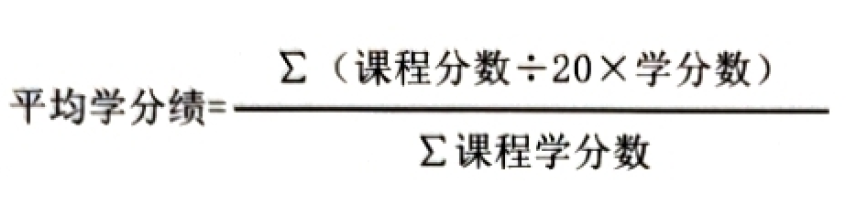
\includegraphics[width=0.5\textwidth]{GPA说明.png}
\end{figure}

\indent 在下文论述中,“可以”表达的是“学生可以选择使用这个GPA去做某事”,这个“可以”达成的条件是数学学院教务处给开成绩证明。
\begin{adjustwidth}{2em}{0pt}
\begin{enumerate}
    \item 全部GPA:顾名思义,即所有课程的GPA。可以用于出国出示;2023年可以用于预推免出示。
    \item 推免综合GPA:推免综合GPA=推免课程GPA+推免加分。推免课程每年\empha{可能会有细微变动},2024年情况(见\cite{推免})如下图,一般仅用于获得推免资格,2024年也可用于预推免出示;推免加分=数学学院认定的加分(见\cite{推免})+学校认定的加分(见\cite{学校加分})。
    \begin{figure}[ht]
    \centering
    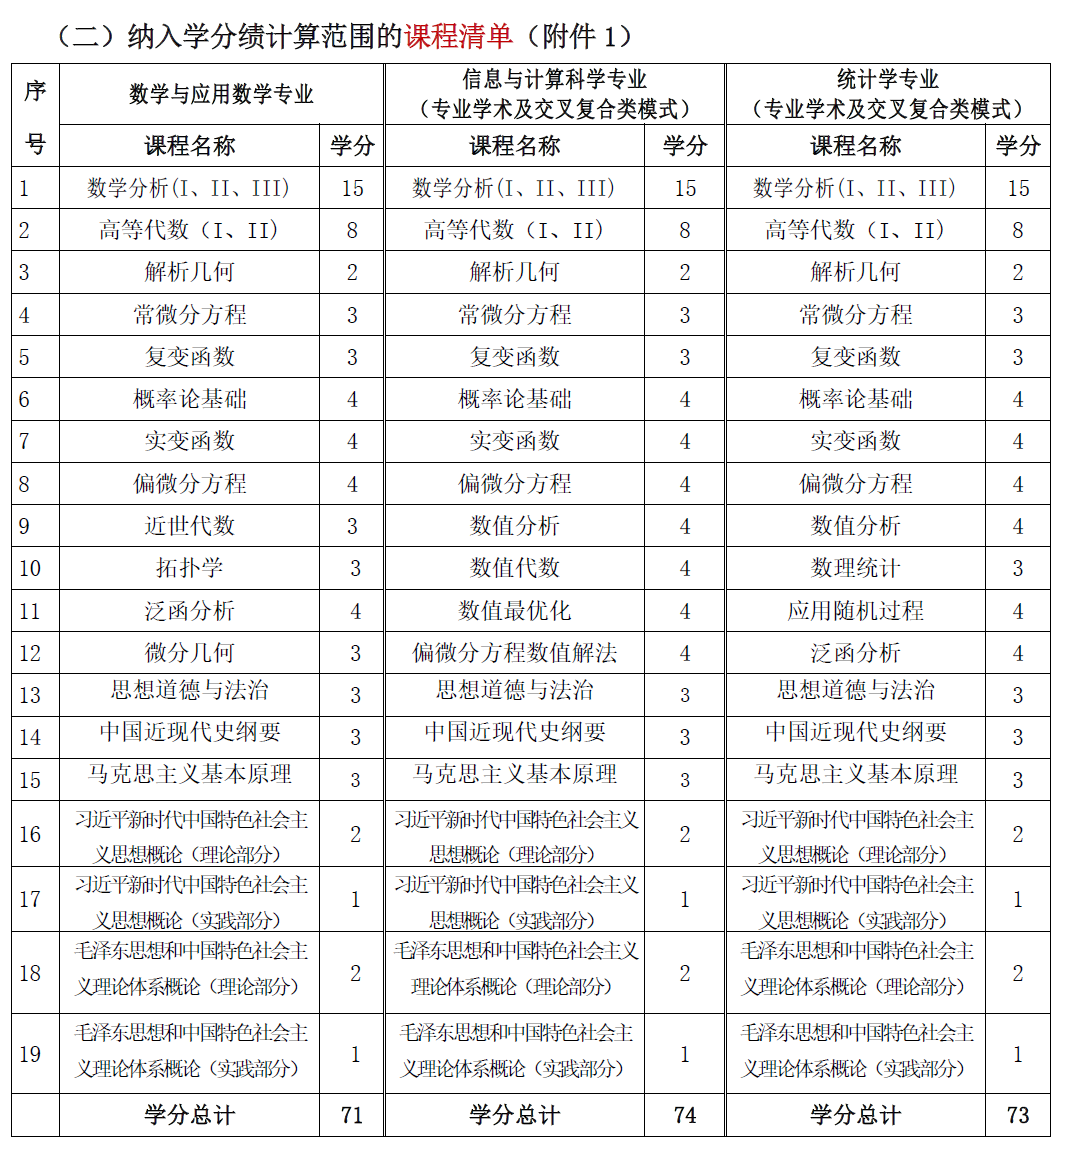
\includegraphics[width=0.5\textwidth]{推免课程.png}
    \end{figure}
    
    \item 核心GPA:亦称滚动课程学分绩,计算除思政外的推免课程的学分绩。是拔尖计划滚动参考GPA,可以用于夏令营、预推免和出国出示。
    \item 学位GPA:也即学位课程学分绩。学位课程为去除掉选修课(数学学院三个专业之间的选修课有细微差别,详见\cite{培养方案})和通识课的所有课程,可以\empha{粗略}地理解为专业课+英语体育+思政课。是评奖评优主要参考GPA,可以用于夏令营、预推免和出国出示。
    
\end{enumerate}
\end{adjustwidth}


\subsubsection{专业课}
毫无疑问,专业课一定是各种GPA中占比均最高的课程,需要报以最大的认真。但是数学专业与许多工科专业最大的不同是,数学专业的课程许多时候并非是“一分耕耘,一分收获”的——在数学的本科学习中,人与人之间智商的差距会进一步地凸显,即使位比在10\%以内的学生,也会感受到自己的努力在别人的悟性前被“羞辱”的感觉。\\
\indent 但智商事实上只决定了每个人的上限,数学有许多专业课还是很靠“勤能补拙”的。大一的\nameref{数分一、数分二}、\nameref{高代一、高代二}是数学四年中都学分占比很高但难度相对较低的课程,如果可以希望同学们能在刚进入大一时便能调整好状态,获得一个好的成绩。大二的\nameref{常微分方程}、\nameref{概率论基础}以及统计专业大三的\nameref{应用随机过程}、\nameref{数理统计}都是靠努力甚至能达到近满分的课程。是如笔者一般的“(相对)笨鸟”先飞的机会。\\
\indent 如果对自己的数学能力非常有自信,只靠核心GPA就能够打遍天下的同学,将专业课学明白就可以了。但对于大多数数学学院的普通人而言,单纯在专业课上“硬碰硬”并非性价比最高的选择。
\subsubsection{英语、体育、思政}
对于“拼刺刀”的核心GPA,提升难度确实较大。但对于学位GPA中的英语、体育、思政课,是都可以通过仔细的红黑榜筛选、认真的课堂课后表现极其有效率地提分的。按照笔者的经验,“卷”这类课程以拉高学位GPA远比“卷”专业课以拉高核心GPA性价比更高。而且学位GPA可以在几乎所有场合平替核心GPA的作用(如\nameref{数学学院GPA概述}所言)。
\subsubsection{其他课程}\label{其他课程}
此外,对于出国的同学,可以通过一些“事少分高”的课程拉高全部GPA。\todo{大家可以补充一些这样的课程}。\\
\indent 关于课程相关知识,我推荐两位学长/学姐撰写的\cite{课程体系},写得非常详细。

\section{发展规划}\label{发展规划}
\subsection{保研}\label{保研}
\subsubsection{保研流程简述}
保研,亦即推免,全称为“推荐优秀应届本科毕业生免试攻读硕士学位研究生”(事实上还有直博)。虽然说“免试”,但是其实只是免除了如考研生一般规范化、制度化的考试,还是需要参加不少院校自己的考核的。\\
\indent 成功的保研由两部分组成:一部分是得到本科所在院校院系(也就是南京大学数学学院)认定的推免资格,推免资格的认定是根据推免综合GPA(详见\nameref{数学学院GPA概述});另一部分是得到研究生接收院校(自然可以是本校)的录取offer。前者保证了你拥有注册国家研招系统的权利,后者保证了你能够在研招系统上填目标院校志愿后被成功录取。\\
\indent 随着推免名额的连年扩张,得到推免名额已经不是难事——2024年数学学院推免名额甚至没有用完,最后保到了推免综合GPA排名101名的同学;但想要得到目标院校的肯定并非易事,保研规划部分也集中在这一部分。\\
\indent 首先需要明确的是,在9月29日国家研招系统上正式录取前,所有院校发的offer均无实质效力,这也就催生出了每年学校鸽学生或学生鸽学校的乱象(“鸽”指的是放鸽子,即承诺会录取/会来但最后爽约),但许多院校的offer都是比较铁的,关于offer效力可以通过公众号、经验贴等得知。\\
\indent 院校各个院系会组织夏令营、预推免和九推来对保研学生进行考核和筛选。夏令营\empha{一般}在7月进行,考核方式比较多样,最后会发“优秀营员”,但此offer每个学校院系效力不一;预推免一般在9月中上旬,考核方式比较固定和传统,得到的初步录取offer被鸽概率小,但许多好的导师可能夏令营期间就已经招满了;九推是929填系统前最后的冲刺,一般是捡漏别人鸽掉的好offer的绝佳机会。要获得学校院系考核内容、考核时间、导师好坏等信息需要保研学生具备信息检索和主动询问/套磁能力,竞争越激烈的院系/方向这场“信息战”的烈度就越高。\\
\indent 由于数学学院保研去向较为多样,且每个方向差别较大,故分别进行陈述。

\subsubsection{基础方向保研规划(完全由2024年保研的王仲祺同学撰写)}
亲爱的学弟学妹们,欢迎大家就读南京大学数学学院!作为一名21级老学长,我十分荣幸能为大家分享一下关于基础方向的保研规划!\\
\indent 进入大学阶段的学习,对于数学系想要保研的同学来说主要可以分为三种:第一种是学术大牛,他们很早就学完了本科甚至是一些研究生课程,积极地参与各种学术活动,平时上课基本看不见人,考试时总是早早答完交卷,从不检查,对于绩点什么的看似毫不关心,却每次都高的吓人。第二种是包括我在内的绝大多数保研人,他们平时绩点在专业里排名靠前,对于数学学习有一些浅显的理解,确立了某一个方向的兴趣,但是因为个人能力问题始终没有付诸于过多的实践,即并没有阅读过多超出必修课的资料,也没有过多涉猎高年级的选修课程,仅仅是能跟上老师的步伐,把每一门必修课做到学明白并掌握。第三种是位于保研边缘的同学,这类同学基本上在保研名单确定以前是不知道自己能保上研的,而名单下来的时候意外地发现了自己有保研名额。由于笔者水平和亲身经历有限,本不能胜任本文的撰写工作,但受老同学之托,在此仅限于讨论第二种情况,即从我自身情况开始讨论,希望能通过自己的经历来为学弟学妹们抛砖引玉,如有叙述不当之处还望海涵!\\
\indent 我们先来聊聊保研的一些准备工作:\\
\indent 首先我认为保研中最重要的就是绩点,虽然我个人并不是唯分数论者,但不可否认的是,绝大多数学校对于绩点排名有着十分苛刻的硬性指标。以我这一年为例,北京大学基本上只给专业前两名(5\% )左右开放面试(我们这一年没有笔试),清华求真书院和复旦大学首批直博生的笔试初审大概卡在年级前15\% 和20\% 左右,中科院的初审要求会根据报名导师和院系的不同而有很大差别,但总的来说会宽松一些。因此总得来看对于绝大多数学校还是对绩点有一定的要求,没有一个合格的绩点排名根本就没有过初审的资格!\\
\indent 我第二个想要强调的点就是打好每一门课的基础,真正掌握了每一门课的思想和精髓,并对里面的理论有一个自己独到的直观理解。可能这时有同学就要问了:“这不是和高绩点一样吗?”非也!绩点绝大多数时候仅仅只能代表你对于题目以及知识点使用技巧的熟练程度,更何况有些课程老师直接从书上课后习题里面出原题,这时绩点甚至只能反映出短时的记忆和背诵能力。而我在这里强调的学会一门课,是指真真正正地理解并运用知识,把所学的抽象概念换成一种直观语言,形成一种独到的见解,理清每一个理论的来由,推导和应用,汇聚成一个整体的思维框架,这样即使你在学完一年甚至两年忘记以后,还依然能通过当年的笔记和书籍快速回忆起来。否则如果第一遍学习的时候就得过且过、自欺欺人,仅仅是通过背题背书背定理来应付考试拿到高分,则在复习时的工作量会大大增加,并且由于想到当年就没学明白,更不愿意花时间钻研,最后估计还是会落个得过且过的下场。\\
\indent 接下来我想说的就是关于兴趣方向的问题,基础数学的大方向一共有以下几个:分析、代数、几何、拓扑、数学物理等等,其中细分的更是数不胜数。在绝大多数保研报名填报的时候,都会要求大家选择某两个方向或者是确定导师进行填报,这就意味着在大三下学期刚开学左右填报时就得确定以后的研究方向,而且在面试的时候老师一定会根据你的研究方向去进行询问,这就要求你在你所感兴趣的方向最好要多学一些内容、多看看一些外国的经典教材,最理想的情况下是在大二或者大一就确定好研究方向,并沿着这个方向一路披荆斩棘、走向数学的无上殿堂!\\
\indent 准备阶段的最后一点就是关于学科竞赛方面,大学阶段能够报名的竞赛有很多,并且绝大多数竞赛相比高中来说门槛实际上是很低的,即不用经过特殊的竞赛训练即可获得部分奖励。这些竞赛包括全国大学生数学竞赛、全国大学生数学建模竞赛、美国大学生数学建模竞赛(美赛)、大学生创新创业训练计划项目(大创)、丘成桐大学生数学竞赛(门槛较高,但重在参与)等等。上述比赛参与基本都能拿到相应奖项,但就是会比较耗费精力,所以如果有空闲时间的话一定要留意各个比赛的报名时间,不要错过哦!\\
\indent 说完了准备阶段,下面来说说关于大三正式开始保研考试的一些建议。\\
\indent 时间上来说,以我这一年为例,是从大三下学期刚开学三月份左右开始的,首先就是北京大学的面试,大概在4月中旬左右,然后就是中科院和清华求真的笔试和面试,大概在5月中旬,然后复旦和清华数学系的笔试在5月末6月初左右。每一个考试大概一周以内就会通知你是否获得优秀营员(或者别的称呼),在收到类似邮件以后不要高兴的太早,一定要向学校和学长确认这个优秀营员是否具有效力,往年是否有鸽学生的例子等等。\\
\indent 关于考试的形式,绝大多数学校都是通过笔试和面试的综合形式进行考查,笔试通过获得面试资格。笔试内容主要部分就是数学分析和高等代数,夹杂着极少量的ode和实变函数。甚至中科院和清华求真的部分面试题仍然是这两门课程。因此在大三下学期开学的时候最好回去细细看一看大一学的这两门专业课,不要有知识上的漏洞。面试内容一般包括两分钟的英文自我介绍(不用学校要求不同)和专业内容考核,其中自我介绍部分建议大三下学期开学就把英汉两种自我介绍都背诵熟练,这样会为后续节约很多时间。专业内容考核各个学校不同,例如北大会问你学了什么东西,你说什么他就会问什么。而中科院计算所则是抽签选题,清华求真则会根据推荐信上面的内容进行提问。\\
\indent 对于面试部分,我建议大家在自己感兴趣的方向能在大二左右多去学习一些,争取能在自由发挥的这部分说出一些有深度的理解,当然如果像我一样什么也没有多学的也不太用担心,老师并不是想看你学的有多么多,而是想看你的理解是否细致是否深刻,况且绝大部分同学都是没多学太多啦,又不是只有你一个你怕什么!\\
\indent 以上就是我个人的保研经验分享啦!希望本文能够为刚踏入大一大二的学弟学妹们关于自己的保研规划有一定帮助,祝愿大家都能进入心仪学府深造,找到自己的理想导师,学习自己的兴趣方向!\\
\indent 难说再见,后会有期!

\subsubsection{计算方向保研规划}

\subsubsection{统计方向保研规划(完全由2024年保研的lwj同学撰写)}
\indent 个人感觉统计是一个很大的方向,我在这里总结的大致是关于理论统计的保研规划,属于统计直博项目。\\
\indent 呢喃数学系的统计在课程体系上和其他统计强校相比知识量是差了很多的。因此在前期的学习中,除了通过统计专业课保证自己的GPA外,建议大家可以多补充一些统计学知识,如回归分析(数理统计课程里的回归分析讲到的内容太少)、时间序列分析、因子分析等。如果未来想要做数理统计方向的同学最好重视数学课程的学习,学有余力可以去选一些基础数学方向的选修课,如拓扑学、微分几何等(流形数据会用到)。\\
\indent 在保研过程中,bg里最看重的我认为是专业知识和编程能力,目前统计领域应用最广泛的还是R语言和python,因此在对bg的准备上除了卷高绩点上,在科研和竞赛经历中体现一下自己的编程能力就可,不必过分看重。夏令营中基本都是笔试加面试(北大的统计科学中心还多一项数据分析项目展示),笔试主要考察数分高代概率论数理统计,面试则会对所有学过的科目进行提问,根据老师的方向大多会问关于实变和随机过程及回归分析的问题。在概率论和数理统计两门课程的复习上,建议使用茆书和李贤平的两本进行系统性复习,概率论要与实变结合,对概念有深刻的理解(如随机变量、密度函数、分布函数和分布等)。统计的专业课中,高绩点不等于好的掌握,因此专业课的复习一定不可马虎。\\
\indent 理论统计里部分的夏令营会有读论文进行展示的环节,如果遇到一定放平心态。往往这几篇论文你是不太可能完全读懂的,基本上放的都是要招生的老师近期的文章。一般先要理解问题是什么,往往结合文章中最后的举例更容易理解,其次要对基本模型有了解,最好不要选择你连基础模型都不懂的文章,这样很难说出有价值的东西。此外在面试中,不论是专业课程还是论文面,一定要诚实!不会就直接说不清楚,或者用其它科目的知识去解释,但一定要对自己说出的定理或证明负责。\\
\indent 夏令营的时间线上,北大光华直博在五月初,北统和清统则分别在五月中下旬,基本上是连着三周。北大光华的bar相对其余要低一些,但是笔试会刷百分之80,笔试内容包括计量经济学和时间序列分析,对于我们的课程体系还是比较困难。笔试过了才可以参加面试,面试则是对读的论文进行ppt汇报。北统分初试和复试。初试为笔试和数据分析项目的PPT展示,都是公开展示,初试通过后会进入复试的论文面,此时为每人半小时左右的单独面试。清统的流程与北统初试一致,但是由于新成立了统计系,后面的考核制度很可能发生变化,且其是强导师制,同学们可以提早联系。北大的老师比较爱压力面,但大家都是压力面,所以同学们一定要抗住!人大和复旦的统计基本上都在暑假,相对前面在笔试难度上有所下降,面试也温和很多。对于夏令营,我倒是觉得大家可以放平心态,以一种交流学习的态度去参与,夏令营本来就是学生和老师相互了解选择的过程。就我个人而言,对于理论统计方向的认识很多都来源于夏令营遇到的同学和老师,眼界着实开拓很多。\\
\indent 以上如果专业实力准备充分,那offer是水到渠成的事情,祝愿大家都能找到自己的兴趣,去到自己的理想项目!
\subsubsection{人工智能方向保研规划}
首先推荐一下2023年保研的ykgg的经验贴\cite{ykgg保研经验贴},里面记述了一些黑话,有助于更好地理解其他经验贴包括笔者的下文论述。\\
\indent 人工智能方向目前还是属于CS方向保研,而随着保研信息的充分交易,CS方向的学生都已经非常明确要卷哪些东西了,导致CS方向保研难度逐年升高。以2024年笔者观察,夏令营阶段各个顶尖AI院系的入营名单重合度极大,整个竞争市场有明显的马太效应趋势。故笔者认为,数学学生与CS方向学生“硬碰硬”地同质化竞争是不现实的,一方面数学专业课已经消耗了许多精力;另一方面数学学院在科研、竞赛等方面的资源和CS院系是无法相比的(再者如果想复刻CS方向保研人的卷法建议本科就转专业)。所以,笔者个人经验是要和CS那帮“怪物”们进行差异化竞争。笔者建议从三个方向着手:\\
\indent 第一是数学本专业的GPA,GPA一般不在意绝对值而看重排名位比(rank,简写为rk)。现实地来说,如果rk较低,你的简历很有可能根本无法出现在你意向导师的面前,而是直接在夏令营/预推免初审阶段就被刷掉。如果你意向导师的方向有理论部分,那一个较高的数学GPA是对你数学基本功的证明;即使你意向做CV等偏工程的方向,较高的数学GPA也是对你学习能力的证明(有相当的老师会认为\empha{连数学都能学好}的学生学其他也会很快)。\\
\indent 量化地来说,2023年的ykgg和笔者说rk在20\%以内就可以在top2以下的除了复旦、人大高瓴以外的的几乎所有夏令营入营(复旦AI并不顶尖但bar奇高),但据笔者2024年保研的体验来说,rk15\%能不能保证入营都是一个未知数,到10\%左右才能说得上很有底气;反而thu颇有一种“不拘一格降人才”的气势,清华AI院2024年甚至会收绩点20\% +,甚至推免名额边缘的学生。不过南大AI院和智科院对于本校生源有保护,目测rk在30\%以内的学生都能过初审,rk即使在50\%以下的学生只要能够联系到老师也能够过初审入营。同时建议要更加认真地学习AI方向应用较多的课程,如统计三大门(概率论基础、应用随机过程、数理统计)和计算方向的优化课程,有时可以弥补在rk方面的相对劣势。\\
\indent 第二是科研经历。一般大家会把科研和竞赛放在同一地位,但是对于数学学生来说,很难拿到一些CS方向的“硬奖项”(如ACM和ICPC等),数学建模比赛(国赛、美赛等)在CS方向保研中个人体会用处并不是很大,所以个人建议可以努力参与,但不需要投入太多期望。\\
\indent 笔者是在大三上的中旬以后才进组接触科研的,但个人觉得还是有些晚。这其中的症结在于笔者“脸皮比较薄”,总是希望能够多把一些基础知识掌握牢固以后再进组,避免被老师和学长认为是废物。但后来才发现,老师和学长们大多数时候并不很care你进组的基础,更看重的是进组以后学习的动力和能力。但诚然,进组前也不能两手空空,必要的基础科研工具(如Python编程基础、数据结构和进组方向的基础知识)是要涉猎的,但并不必要掌握得非常牢固,\empha{进组后要用啥学啥是效率最高的}。从保研结束后的复盘来看,笔者认为如果能够早早确定对AI的兴趣,在保证GPA能够达标的基础上越早进组越好,能够本科发表出一篇顶会整个保研之路会畅通非常多。在确认了科研兴趣或者想做一些兴趣探索的基础上,可以通过询问学长学姐(可以在qq群:856910513中找到南大数学转AI的一些学长学姐)来选择好的老师,直接通过邮箱/线下等方式联系进组;也可以利用一些契机,如大创和一些比赛,联系感兴趣的课题进行科研启蒙。进组以后由于基础薄弱,学长可能会安排你只干一些杂货,这就考验自己的交流能力和主观能动性:多主动要机会,多提出自己的思考,多构建对这个方向的理解,慢慢加入核心工作,而非学长安排什么就\empha{只}做什么。不过确定兴趣这点其实是很难的,这就引出了第三点需要努力的方向。\\
\indent 第三是对AI整个方向的理解和兴趣,最好能够对某一个小方向有浓厚的兴趣。许多数学学生选择数学本科,其实并不对数学有多么浓厚的兴趣,更多地是如笔者一般基于对自己兴趣的不确定和对于未来的茫然,希望一边学一门“硬手艺”傍身一边不断探索。所以,笔者建议在大一和大二一定要从繁忙的课程中挤出时间,进行对各种数学以外的知识的广泛涉猎,以明确自己的志向所在。笔者在附录推荐材料\nameref{AI推荐材料}中记录了笔者亲身上过的课程和阅读过的书籍,有的可能需要一些基础,但可以边看边学。\\
\indent 如果能够对某一方向有浓厚的兴趣,不妨立足于此开展科研工作,毕竟兴趣是最好的老师。在保研过程中,数学学生应着力于强调“我的数学功底能够帮助我在此领域有所优势、我的CS技能已经够用、我对这个方向兴趣斐然”。如若找不到自己感兴趣的方向,也不妨调整最后一部分为“我对于AI领域涉猎颇多”。如此使用差异化的策略方能避免与CS佬们的直接冲突,更能让老师看到你的闪光点,更详细的可见笔者的保研经验贴\cite{笔者的保研经验贴}。

\indent 此外,数学学生还要注意保研中某些营是有机试的。机试一般分为两种,第一种是算法机试,也就是Leetcode题,这里推荐Acwing算法基础课和Leetcode hot100练习进行学习和巩固,学明白这两个足以应对top2以下的算法机试了;第二种是机器学习机试,目前只听说过我们敬爱的母校AI学院会考察这个,一般是让你补全或撰写机器学习代码,推荐头歌平台机器学习课程进行练习。

\subsubsection{金融方向保研规划(完全由2023年保研的巫天骐同学撰写)}
首先,我们按照流行的说法对一些top级别的金融项目做一个排序,然后再对各个项目分别做一个简单的介绍(具体信息可以参照对应学院的官方网站,或关注经管保研公众号“保研声”)。

~\\
\\T0:北大光华,清华经管(北京)
\\T1: 上交高金,清华五道口
\\T2: 复旦泛海,复旦管院,北大汇丰,北大数院,清华经管(深圳)
\\T3:上交安泰,人大财金,复旦经院,北大软微~\\

T0和T1档对学生的要求是相当高的,绩点rank在整个数院前3并且拥有很高title的实习或项目经历可以考虑冲一冲(数学系之前好几年才会出一个)。

复旦管院有两个很吃香的专硕项目,分别是dsba(数据科学与商务分析)和mfe(金融工程),入营难度相对较低,rank在20\%左右的同学也基本能够有资格参加笔试,但是由于竞争激烈、面试难度比较大,所以拿到offer还是一件相对困难的事。之前的面试中,有学长被问到机器学习中的ROC曲线是什么,如何解决多元线性回归中的多重共线性问题这类偏应用的问题。该项目的学费比较贵,学制为两年,学费每年10.8w(可能会变化,具体参考学院官网),没有住宿,不过相比项目含金量来说还是非常值得的。

北大汇丰是一个偏学术的项目,它对绩点会更卡一些。保研进入该项目会分两个批次,分别是7月的夏令营和9月的预推免。排名在5\%之前进入夏令营会比较稳,排名在10\%之前进入预推免会比较稳。参加夏令营需提交一篇参营论文,并在现场进行论文答辩,答辩完成后还有面试的考核,而预推免只有20分钟的面试考核。考核均为全英文。夏令营往年的通过率达到了80\%,预推免通过率只有夏令营的一半甚至不到。如果数学系的同学在大三暑假阶段还没有科研论文产出的话,可以等9月份报名预推免冲一冲。该项目学制为三年(第一年禁止实习,第二年禁止离开深圳实习,入学前有为期一周的封闭式军训,管理较为严格,毕业也有一定学分绩要求),学费每年4.6w,深研院提供宿舍。

上交安泰不光有金融硕士项目的专硕,也包含数学人常去的管理科学与工程专业的学硕,并且安泰近几年在管科方向的发展势头非常猛,绩点在专业前15\%内入营会比较稳。如果有想往运筹方向走的同学可以准备该方向的学硕营。考核包含一小时的逻辑题笔试和20分钟的面试。学硕的学制为2.5年,学费是8000/年,并且安泰提供在徐汇校区的宿舍,对于找实习是非常方便的。

上面列举了一些常见项目的特点,笼统地概括一下:金融项目的面试往往不会如同数学项目要求在黑板做题、考察很深的数学知识等,而是问得很发散、很应用,比如research ideas,常用机器学习算法,对量化行业的了解等等。下面我接着说一说,如果想从南大数学系转行金融领域应该早些做好的几点准备:

1.代码能力。重中之重,很多跨保金融的同学基本都是朝着量化方向发展的,而量化策略的实现离不开代码。业界的主流语言是Python,如果能会C就更好。Python中尤其重视pandas, numpy库的学习,学有余力可以学一学Python的深度学习模块,即TensorFlow或PyTorch。在学习过程中尽量用向量化方式编写函数,减少loop的使用,因为在实际处理股票数据的时候效率很重要。

2.项目经历。做项目一定是基于代码能力之上的,比如全国大学生建模竞赛、美国大学生建模竞赛等,或者在Kaggle网站自己进行比赛复现。如果外院系有合适的大学生创新创业项目也可以跟着做。周志华老师在计算机学院每年都会开设《机器学习》课程,课程大作业就是一次Kaggle比赛任务,这样的比赛如果获得了好名次,是绝对可以丰富简历的。我们系的某些课程也有“大作业”的设置,如《数理统计》《数据分析》等,不过分数占比小、编程要求低,很多同学即使水过去也不会对总评产生太大影响,但是长远看来,如果说想增加简历中的项目经历,那还是要抓住这为数不多的机会好好做一下。

3.实习经历。做实习可以说是建立在前两点之上,即如果对Python等语言拥有比较扎实的掌握,并且已经拥有含金量较高的项目经历,可以试着投一投有一定规模的买方私募。卖方的要求会相对低一些,这里我比较推荐想转金融的同学在大二/大三的某学期选上郑钢老师开设的1学分公选课《郑钢证券行业研究训练营》,这些课程一般都会邀请各大券商研究所的首席分析师来给大家介绍目前该行业的情况,对拓宽视野、进一步了解金融市场非常有帮助,还可以在嘉宾介绍结束之后投对应行业的实习(一般不会收到拒信,并且线上实习即可,不过缺点是没有工资)。主攻量化的同学可以由券商金融工程组开始起步和接触量化。

上述三点就是一些准备金融项目保研的建议,第一点可以充分利用大一和大二的假期完成,第二点和第三点可能要求同学们在平时多付出一些数学课之外的时间。不过,即使是这三点都没有,一个很高的绩点在T2的很多项目中也是够用的,但是保研结束后最好趁大四赶紧补上。

\subsection{出国(几乎完全由申请25 fall留学的浅冽撰写)}
以下部分完全由2024年申请出国的lyt同学撰写,同时笔者需要补充的是,各院系每年民间编纂的\empha{飞跃手册}是了解该年学长学姐出国去向和经验的好材料。
\subsubsection{成绩方面}

\textbf{学分绩的计算}:出国申请时,学校看的是你的全部学分绩和学位学分绩中较高的那个。这与国内保研只看单一保研学分绩不同,因此你可以通过选择多门给分较好的选修课来提升整体成绩。

\textbf{选修课策略}:在选择选修课时,建议参考《选课红黑榜》,该榜单里有关于大多数课程的考核方式、给分难易、任务多少等评价。可以优先选择不需要签到、只需提交一篇大论文的课程,适合那些打算出国的同学。

\textbf{WES成绩的影响}:部分美国学校可能会要求提交WES成绩,该成绩是根据课程与专业的紧密关系进行加权的。因此,选择与自己专业相关的选修课也很重要。

\textbf{退课和重修}:国外大学对于退课和重修的记录不会过分关注,尤其是如果你已经决定出国,建议在大二和大三期间对不满意的课程进行重修。如果某门课感觉难度过大,即便过了学期的第二周,也可以考虑直接退课。

\subsubsection{交换经历}

\textbf{交换的重要性}:交换经历在出国申请中有很大帮助,具体收获包括但不限于:
\begin{itemize}
    \item 获取一份国外学校的成绩单,这通常比国内成绩更受认可。
    \item 有机会获得国外教授的推荐信,这在国外申请中更具优势。
    \item 语言能力的提升,尤其是英语水平会有大幅提高。
    \item 获取参与国外科研项目的机会,虽然难度较大,但非常有助于申请。
\end{itemize}

\textbf{交换经历建议}:建议计划出国的学生至少有1-2段交换经历,最好是1段短期交换和1段长期交换的组合。

\subsubsection{其它申请因素}

\textbf{科研经历的重要性}:好的科研经历相当于强推荐信,往往比单纯的GPA还要有分量。因此,科研成果并非唯一评价标准,关键是要有实际参与的科研经验。

\textbf{推荐信}:强有力的推荐信在申请中非常重要,尤其是来自科研导师或国外教授的推荐信。

\textbf{优先级顺序}:出国申请中的优先顺序大致为:好的科研经历 = 强推荐信 > GPA > 一般科研或推荐信或实习 > 语言成绩 > 课外活动与工作经历(理工科专业基本不看,商科和文科可能会看一些)。

\subsection{考研}\label{考研}

\subsection{就业}\label{就业}

\section{数学学院课程指导(红黑榜)}\label{红黑榜}
数学学院有自己的github资料仓库,其中有往届学长学姐整理的往年卷等资料:\href{https://github.com/will-c137/TG-files.git}{TG-files}。同时,zjc同学也自己整理过\href{https://tg0.gitbook.io/tgbook}{南数课程指南}(不过已经停止维护),欢迎大家参考。\\
\indent 总的来说,笔者个人认为统计是三个专业中给分相对最高的,但笔者强烈建议当有强烈偏好的情况下一定要顺从个人的兴趣,不然大三大四学习会非常痛苦。
\subsection{数分一、数分二}\label{数分一、数分二}
2021年mjq老师:为了避免大一就把学生都吓得不敢分流到数学(bushi,数分一、数分二难度并不大,基本“学懂”并不非常困难,但笔者认为需要考一个高分还是需要一定的做题熟练度的——熟练度的训练只需要把课上例题和课后习题反复消化就够。对于希望打牢基础/挑战自身能力的同学,可以尝试谢惠民,但不需要过于执着,做不出来并不代表学不好今后的数学。
\subsection{高代一、高代二}\label{高代一、高代二}

\subsection{数分三}
2022年md老师:苗老师的讲课风格还是非常有特色的,但想考好并不需要将苗老师讲的拓展内容全部学会。此年苗栋老师期中考试出卷非常之困难,让许多天赋较好的同学都“心如缟素,面如死灰”,希望大家能够撑住……

\subsection{常微分方程}\label{常微分方程}

\subsection{数值分析}
2024年dwb老师:笔者上机作业github仓库:
\href{https://github.com/Chenruishuo/Numerical-Analysis-in-Nanjing-University.git}{Numerical-Analysis-in-Nanjing-University}。

\subsection{概率论基础}\label{概率论基础}
2022年dxp、syl老师:期末考试时syl老师很详细地复习了一波,并且复习题中有考试原题。期中考试与往年卷重合度很高,刷明白往年卷即可。

\subsection{应用随机过程}\label{应用随机过程}
2023年dxp老师:期中期末考试基本均是老师讲义上的原题以及简单变体和定理,理论上把整个讲义背下来就能满分。注意很长的定理证明也有可能会考到,此年考试就考了讲义上最长的定理证明。
\subsection{数理统计}\label{数理统计}
2023年wlh老师:期中期末考试与往年卷重合度极高,所考察的方法几乎完全一样,认真复习两遍书并刷完往年卷95+不难。

\section{未来完善方向}
这本册子作为笔者和其他撰写者的某种意义上的“作品”,我们真心希望它能够作为一个载体,促使信息不断从“前人”流向“后人”,故希望今后能有包括但不限于以下完善:
\begin{itemize}
    \item 希望\nameref{保研}一节中能够补充“计算方向保研规划”,笔者找到的本级计算方向同学实在太强,不如何需要规划就能轻松上岸。
    \item 希望\nameref{其他课程}中能够补充一些“事少分高”的课程。
    \item 希望\nameref{红黑榜}能够成为数学学院自己的红黑榜,各种课程信息能够更加具体和跟上变化。
    \item 希望\nameref{发展规划}中\nameref{考研}和\nameref{就业}规划得以补充。
    \item 希望大家可以多多贡献自己所知道的信息,建议在希望补充的小节末尾以“【称呼】:【所要补充的信息】”格式进行撰写。对于希望重写一篇的(如希望撰写自己的“基础方向保研规划”),可以另开小节(如“基础方向保研规划二(完全由xxxx年保研的xxx同学撰写))”。
\end{itemize}

\section{致谢}
感谢zqc同学对本生存手册关于数学强基政策内容的支持。感谢yzh、ghk、jlx、lzy同学对\nameref{进入数学学院面试案例}的贡献。感谢zjc等同学对于数学学院github仓库的维护。感谢ykgg等学长学姐对包括笔者在内的一众学弟/学妹的帮助。感谢愿意留下联系方式的编者,见\nameref{部分编者联系方式}。\\
\indent 最后感谢所有将来为此手册添砖加瓦的同学们,希望大家都能在南京大学数学学院的本科学习和生活中不留遗憾。


\printbibliography

\newpage
\section*{附录}
\begin{appendices}
\section{进入数学学院面试案例}\label{进入数学学院面试案例}

\subsection{拔尖面试}\label{拔尖面试详细}
\begin{adjustwidth}{2em}{0pt}
\begin{enumerate}
    \item yzh:问了我三个问题:(1)你学过数学分析吗?(2)你学过高等代数吗?(3)你为什么会来考数拔?一般是一个教分析的老师一个教代数的老师和吴婷来面试。他会问你学过啥,然后根据你说的问一些问题。比如邱华让我描述Cauchy收敛准则,朱富海问我什么样的多项式可以因式分解。
\end{enumerate}
\end{adjustwidth}

\subsection{大类分流面试}\label{大类分流面试详细}
\begin{adjustwidth}{2em}{0pt}
\begin{enumerate}
    \item ghk:(目前已经大三了所以有些细节记不清楚)大类分流面试,教室里有三个老师,当时面试我的是cw老师,gxj老师,另一位不认识.面试全程中文.面试开始后先进行一段自我介绍.随后cw老师说(大意是)你已经学习过数学分析高等代数解析几何,你的学习情况如何.随后问什么是微积分基本定理(当时脑子没转过来,另一位老师提醒就是Newton-Leibniz公式)陈述完定理表述(当时我假设被积函数是连续函数)cw老师又问这个公式有什么用.我一开始回答可以简便积分计算,cw老师要求说得更实在一些,不要说这些虚的东西.于是我用Newton-Leibniz公式推导了Lagrange中值定理.接下来我被问及Newton-Leibniz公式是否有高维的推导,我回答Green公式Gauss公式Stokes公式,并被要求写出来(当时选择了Green公式).最后gxj老师问如何判断一个矩阵方程有解,回答后又追问何时有唯一解.此时我的回答是“行列式不等于零”,gxj老师进一步追问如果矩阵不是方阵该如何判断. 大致就是这些了,面试过程全程允许使用黑板.
    \item jlx:我记得当时先做个自我介绍,问问数分高代哪个更喜欢,哪个花的时间更多,然后会根据你说的问接下来的问题。问我的是“有界闭集是什么”“实数系基本性质还记得吗,会互推吗”“有限覆盖定理是什么,条件能减弱吗(我没懂”,高代问了jordan标准型那一部分的思路,然后就over了.
\end{enumerate}
\end{adjustwidth}

\subsection{转专业面试}\label{转专业面试详细}
\begin{adjustwidth}{2em}{0pt}
\begin{enumerate}
    \item lzy:(大二下转专业)我的分为数分高代俩部分,先问我擅长啥,然后从擅长的说起,数分问的是黎曼函数定义,间断点有什么,类型分别是,为什么是间断点,其他记得不太清楚,高代部分是Jordan标准型(这个甚至给了我的具体的矩阵让我想他的标准型是什么,比较简单的矩阵),第二空间分解定理陈述,特征值,特征子空间,大体就记得这么多[表情]
\end{enumerate}
\end{adjustwidth}
\section{推荐材料}
\subsection{金融方向}
\subsubsection{课程}\label{金融推荐课程}
\begin{adjustwidth}{3em}{0pt}
\begin{enumerate}
    \item 走进金融业:会请到许多金融各行各业的人士来讲述从业心得,并进行交流。是一个大致了解金融行业组成和业务的窗口。
    \item 郑钢证券行业研究训练营:由校友郑钢先生组织,邀请到许多券商首席分析师进行各投资行业的解读,可以具体了解二级行业研究。
    \item 认识中国:老师讲课很有水平,会讲改革开放后的经济政策,是一个从理解中国经济发展历史的机会。
\end{enumerate}
\end{adjustwidth}

\subsubsection{书籍}\label{金融推荐书籍}
\begin{adjustwidth}{3em}{0pt}
\begin{enumerate}
    \item 《经济学原理》,曼昆:是一本入门经济学的简单书籍。
    \item 《货币、银行和金融体系》,格伦哈伯德:顾名思义,是一本建立金融体系认知的书籍。
    \item 《金融经济学二十五讲》:是一本数学基础要求很高的金融经济学书籍,可以一窥数学到底在金融学中有何用武之地。
\end{enumerate}
\end{adjustwidth}

\subsubsection{其他资源}
\begin{adjustwidth}{3em}{0pt}
\begin{enumerate}
    \item b站up主\, 有何高见9527:是我个人认为分析比较客观的财经up主,可以通过他的分析边听边学一些金融实务的基础知识。
\end{enumerate}
\end{adjustwidth}

\subsection{AI方向}\label{AI推荐材料}
\begin{adjustwidth}{2em}{0pt}
\begin{enumerate}
    \item 《机器学习》,周志华:同时推荐AI院的“机器学习导论”课程。此书是南京大学AI院夏令营考核的重要参考书籍,里面介绍了偏传统机器学习的各个方向,是一本入门机器学习并为转南大AI做准备的好书。
    \item 《动手学深度学习》,李沐等:可以直接使用\href{https://zh.d2l.ai/}{网页版}以更方便地运行其中的代码。是一本立足于代码手把手教你入门深度学习的好书。
    \item 《人工智能 现代方法(第四版)》:同时推荐AI院的“人工智能导论”课程。可以通过此书(课程)了解较为现代的人工智能进展。
    \item 《数据结构(C++语言版 第3版)》,邓俊辉:数据结构是CS方向的最基础课程。邓俊辉老师的书结合图片,讲解很清晰,习题也很有深度(故如果有时间建议再买一本习题解析),同时此本书配套有学堂在线上的网课和pdf资料。邓俊辉老师本人也很有魅力,受他的感召笔者的PPT每个封面都要带一句能够表达本节思想的话。
    \item \href{https://www.runoob.com/}{菜鸟教程}:是一个用来学习编程语言的网站,突破了教科书全是定义的枯燥,更加立足于“会用”“能跑”,能帮助学生快速上手编程语言。
    \item \href{https://hrl.boyuai.com/}{动手学强化学习}:强化学习是一个和数学结合紧密,并且笔者个人认为应用潜力较大的机器学习方向。此书(网站)立足于代码和经典论文,让人感受到RL的魅力。此外,这个系列还有一些《动手学XX》可供XX领域的代码入门。
    \item \href{https://cloud.tsinghua.edu.cn/d/2176225b8d904d1d9441/}{清华叉院强化学习课程}:是知名学术/创业新星许华哲老师的强化学习课程,很接轨时代,推荐。
\end{enumerate}
\end{adjustwidth}

\section{部分编者联系方式}\label{部分编者联系方式}
\begin{adjustwidth}{2em}{0pt}
\begin{enumerate}
    \item 陈睿硕(笔者):\{邮箱,\href{mailto:ruishuochen@163.com}{ruishuochen@163.com}\}
    \item 唐晨皓:\{邮箱,\href{mailto:370052012@qq.com}{370052012@qq.com}\}
    \item 王仲祺:\{邮箱,\href{mailto:18809855111@139.com}{18809855111@139.com}\}
    \item 巫天琪:\{微信,wizard\underline{ }0820\}
    \item 浅冽:\{邮箱,\href{mailto:2110934387@qq.com}{2110934387@qq.com}\}
    \item lwj:\{邮箱,\href{mailto:738582691@qq.com}{738582691@qq.com}\}
\end{enumerate}
\end{adjustwidth}
\end{appendices}

\end{document}



